\documentclass{report} 
\usepackage[a4paper, total={7in, 10in}]{geometry}
\usepackage{graphicx} 
\usepackage{xcolor} 
\usepackage{amsmath} 
\usepackage{amsfonts} 
\usepackage{mathtools}
\usepackage{listings}
\usepackage{caption}
\usepackage{ragged2e}
\usepackage{hyperref}
\usepackage{soul}
\usepackage{multirow}
\usepackage{booktabs}
\usepackage{array}
\usepackage{pgfplots}
\usepackage{tikz}
\usepackage{amssymb}
\usepackage{transparent}
\usepackage{enumitem}
\usepackage{footnote}
\usepackage{footmisc}

\pgfplotsset{compat=1.18}
\definecolor{dark-green}{RGB}{0, 100, 0}

\lstset{
    basicstyle=\ttfamily\small,   
    morekeywords={sig, freqsig, f_low, f_high,signal, Nf}, 
    keywordstyle=\color{blue},
    stringstyle=\color{dark-green},     
    frame=none,             
    numbers=none,           
    breaklines=true,        
    showstringspaces=false,
    backgroundcolor=\color{white}
}

\lstset{emph={energia_media_f}, emphstyle={\color{red}\bfseries}}

\captionsetup[figure]{labelformat=empty}
\justifying

\renewcommand{\thefootnote}{\fnsymbol{footnote}}

\renewcommand{\thesection}{\arabic{section}}
\setcounter{section}{0}
\renewcommand{\thefootnote}{\arabic{footnote}}

\title{\textbf{Report Homework FCI I - Gruppo 2}}
\author{Davide Gaglione\footnote{Rappresenta il gruppo in qualità di leader.}, Andrea Carbone, Alessandro Chitarrini e Matteo Crugliano}
\date{}

\begin{document}

\maketitle

\section{Definizione di segnali e grafici}

\textit{Caricare il file trovato nella cartella “eeg\_CP4\_MI\_LH\_s01.mat” tramite la funzione loadmat. Il segnale è relativo al soggetto 1 mentre effettua il task di Motor Imagery della mano sinistra (Motor Imagery Left Hand). Si tratta del segnale registrato al sensore CP4. Considerare il segnale discreto soltanto nei campioni compresi tra $n1=500$ e $n2 =2500$. Il passo temporale tra un campione e il successivo è di 2 ms. 1. Fare il grafico del segnale $x_n$; 2. Calcolare l’energia di $x_n$ e scriverla in un box all’interno del grafico precedente.}

\begin{figure}[!h]
\begin{minipage}{0.4\textwidth} 
Per prima cosa, abbiamo importato il file \texttt{eeg\_CP4\_MI\_LH\_s01.mat} utilizzando la funzione \texttt{loadmat()}\footnotemark, che consente di caricare i dati da un file MATLAB. Il file contiene un segnale EEG registrato dal sensore CP4, relativo al soggetto 1 durante l'esecuzione del compito di \textit{Motor Imagery} della mano sinistra. Dopo aver estratto il segnale, ci siamo concentrati unicamente sui campioni compresi tra $n_1 = 500$ e $n_2 = 2500$. Considerando un passo temporale tra i campioni pari a $t = 0.002 s$ ($2 ms$). In merito è stato possibile realizzare un asse temporale in secondi (raggiungendo un tempo totale analizzato di $4 s$), necessario per rappresentare correttamente il segnale in funzione del tempo. Successivamente, utilizzando la funzione \texttt{plot()}\footnotemark, abbiamo \textbf{rappresentato il segnale $x_n$} in funzione del tempo (visibile nella figura a destra). Infine, in questa prima sezione, abbiamo \textbf{calcolato l'energia} del segnale, definita come $E = \sum_{n=n_1}^{n_2} x_n^2$ e riportato il valore calcolato in un riquadro all'interno del grafico.
\end{minipage}
\hfill
\hspace{0.5cm}
\begin{minipage}{0.55\textwidth}
\centering
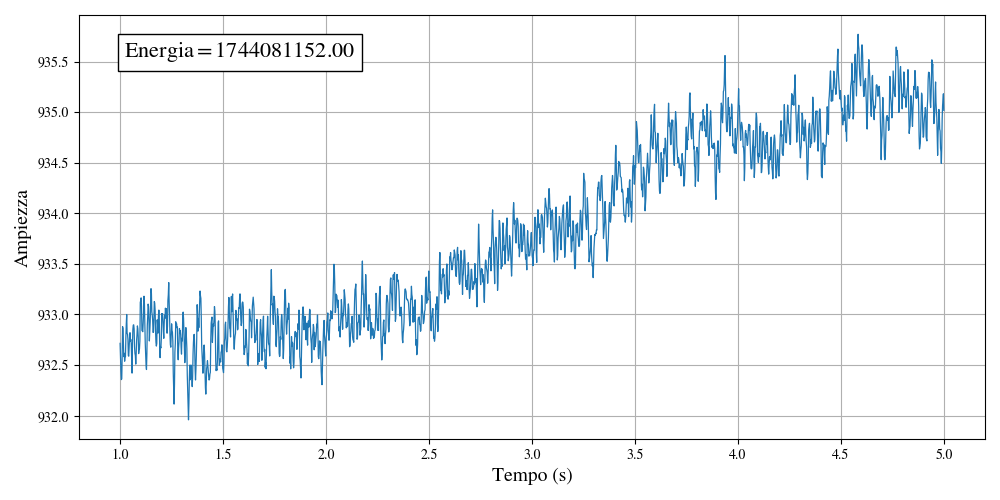
\includegraphics[width=\textwidth]{plot1}
\caption{Segnale EEG del soggetto 1: Motor Imagery Left Hand (CP4)}    
\end{minipage}
\end{figure}

\footnotetext[1]{della libreria \texttt{scipy.io}.}
\footnotetext[2]{della libreria \texttt{matplotlib.pyplot}. Abbiamo scelto questa funzione in alternativa a \texttt{stem()} per migliorare la leggibità.}

\section{Studio di una coppia di segnali}

\textit{Caricare il file trovato nella cartella “eeg\_C4\_MI\_LH\_s01.mat”. Si tratta del segnale registrato dallo stesso soggetto per lo stesso task in corrispondenza del sensore C4. 3. Prendere il segnale soltanto nei campioni compresi tra $n1=500$ e $n2 =2500$. Il
passo temporale tra un campione e il successivo è di 2 ms. Calcolare il valore medio
di questo segnale e sottrarlo ai valori del segnale. Rappresentare il grafico di questo
segnale $y_n$ (a cui è stato sottratto il suo valore medio); 4. Calcolare il coefficiente di correlazione tra il segnale originario $x_n$ e $y_n$.}

\begin{figure}[!h]
\begin{minipage}{0.4\textwidth}
In questa seconda sezione abbiamo analizzato un altro segnale, questa volta registrato dal sensore C4 durante lo stesso esperimento per la mano sinistra. Il segnale è stato considerato nello stesso intervallo $[n_1,n_2]$ e passo ($t$) del primo sensore (CP4). Successivamente, abbiamo calcolato il valore medio del segnale e lo abbiamo sottratto da ciascun valore del segnale originale, ottenendo così il segnale graficato ($y_n$). Il passo successivo è stato il calcolo del coefficiente di correlazione tra il segnale $x_n$ e il segnale $y_n$ utilizzando la funzione \texttt{corrcoef()}\footnotemark. Tale valore è pari a:

$$\boxed{ \rho_{x_ny_n}= 0.45150673558168236}$$
\end{minipage}
\hfill
\hspace{0.5cm}
\begin{minipage}{0.55\textwidth}
\centering
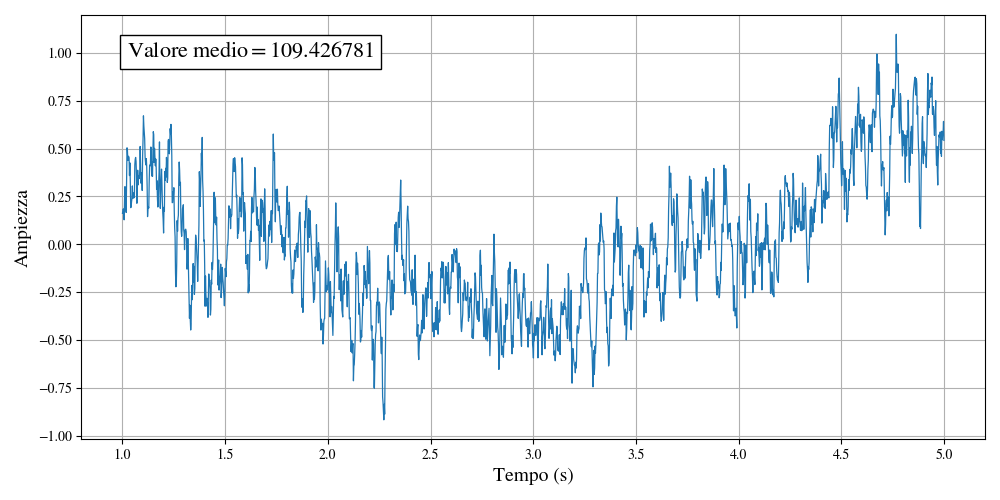
\includegraphics[width=\textwidth]{plot2}
\caption{Segnale EEG del soggetto 1: Motor Imagery Left Hand (C4)}    
\end{minipage}
\end{figure}

\footnotetext[3]{della libreria \texttt{numpy}.}

\section{Studio del segnale in frequenza}

\textit{5. Calcola la trasformata di Fourier del segnale $x_n$ usando la fast fourier transform (fft). Generare il vettore delle frequenze con fftfreq. Visualizzare il valore assoluto della trasformata di Fourier tramite fftshift. 6. Applicare un filtro passa banda nelle frequenze comprese in $\alpha=[8,13]$ Hz. Rappresentare la risposta in frequenza del filtro e l’uscita del filtro nel tempo $z_n$.}

\begin{figure}[!h]
\begin{minipage}{0.4\textwidth}
	Il segnale $x_n$ è stato analizzato nel dominio della frequenza utilizzando la \textbf{trasformata di Fourier} discreta (\texttt{fft()}\footnotemark). Dopo questo passaggio abbiamo generato il \textbf{vettore delle frequenze} con la funzione \texttt{fftfreq()\footnotemark[4]}, questo processo ha permesso di convertire il segnale dal dominio temporale a quello delle frequenze, consentendo di osservare come l’energia del segnale sia distribuita tra le diverse componenti frequenziali. Il modulo della trasformata è stato visualizzato dopo aver \textbf{centrato lo spettro} con l’operazione di \texttt{fftshift()}\footnotemark[4], come visibile nel grafico a destra.
\end{minipage}
\hfill
\hspace{0.5cm}
\begin{minipage}{0.55\textwidth}
\centering
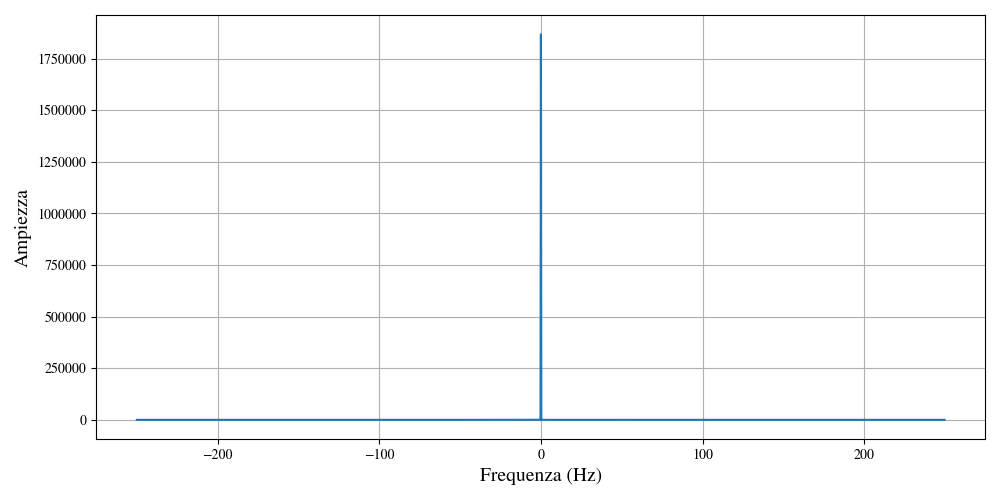
\includegraphics[width=\textwidth]{plot3}
\caption{Valore assoluto della trasformata di Fourier}    
\end{minipage}
\end{figure}

\begin{figure}[!h]
\begin{minipage}{0.4\textwidth}
	Per isolare una specifica banda di frequenze, abbiamo progettato un \textbf{filtro passa banda} ideale (\texttt{ideal\_filter()\footnotemark}), definito per lasciar passare solo le frequenze comprese tra 8 e 13 Hz. Questo filtro è stato implementato come una funzione a gradino che assume valore unitario nella banda desiderata e zero al di fuori. La sua \textbf{risposta in frequenza} $H(f)$ è stata graficata per confermare la selettività del filtro, come visibile in figura. Questo passaggio è cruciale per rimuovere componenti indesiderate dal segnale originale e preservare solo quelle di interesse. L’analisi del filtro è stata eseguita verificando il suo comportamento sullo spettro delle frequenze.
\end{minipage}
\hfill
\hspace{0.5cm}
\begin{minipage}{0.55\textwidth}
\centering
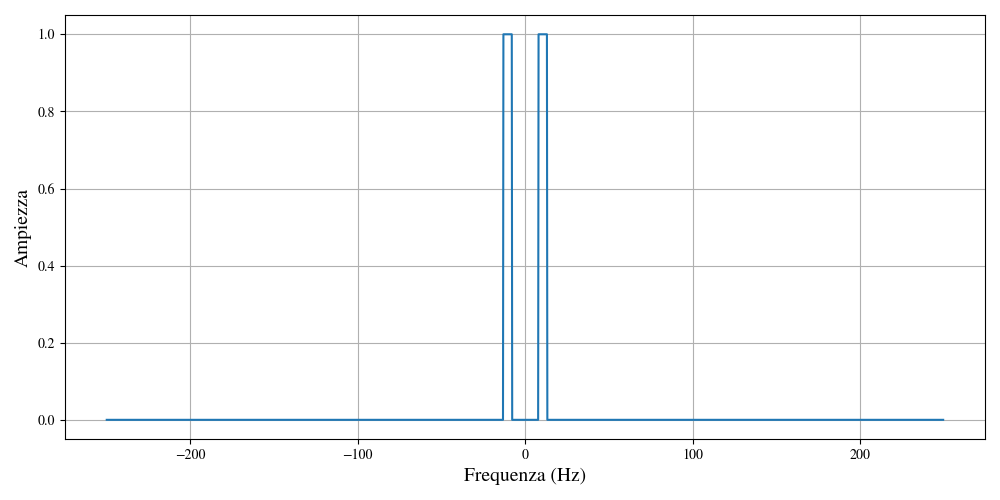
\includegraphics[width=\textwidth]{plot4}
\caption{Risposta in frequenza del filtro passa banda}    
\end{minipage}
\end{figure}

\begin{figure}[!h]
\begin{minipage}{0.4\textwidth}
Successivamente, il filtro passa banda è stato applicato al segnale trasformato nel dominio della frequenza moltiplicando lo spettro $X(f)$ per la risposta del filtro $H(f)$. Questo passaggio consente di eliminare tutte le componenti frequenziali esterne alla banda compresa tra 8 e 13 Hz, preservando unicamente le frequenze desiderate. Il risultato, $Y_{BP}(f)$, rappresenta lo spettro filtrato. Attraverso la trasformata inversa di Fourier, calcolata con la funzione \texttt{ifft()\footnotemark[4]}, $Y_{BP}(f)$ è stato riportato nel dominio del tempo, ottenendo \textbf{l'uscita del filtro nel tempo} $z_n$, depurato dalle frequenze indesiderate, come visibile in figura.
\end{minipage}
\hfill
\hspace{0.5cm}
\begin{minipage}{0.55\textwidth}
\centering
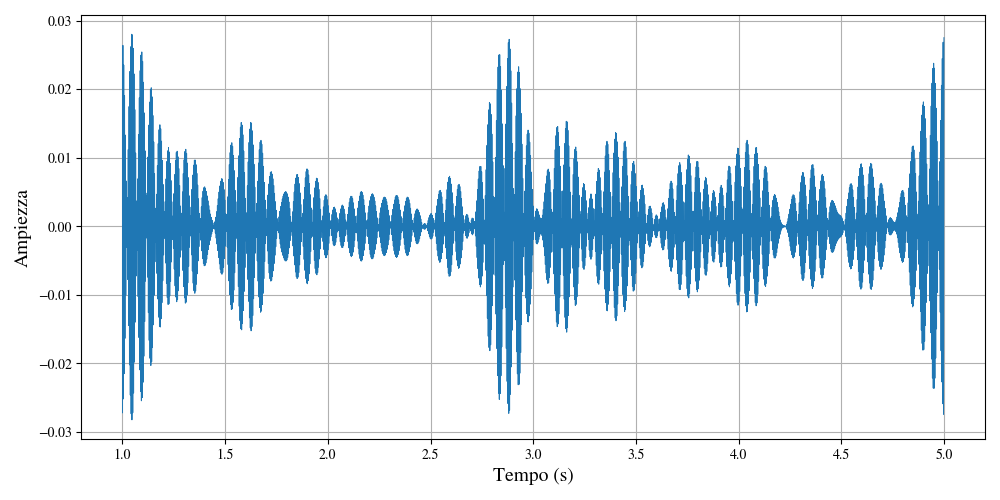
\includegraphics[width=\textwidth]{plot5}
\caption{Uscita del filtro nel tempo $z_n$}    
\end{minipage}
\end{figure}

\footnotetext[4]{della libreria \texttt{scipy.fft}.}

\footnotetext[5]{
\texttt{ideal\_filter(sig, freqsig, f\_low=None, f\_high=None):}\\
    \indent\texttt{\hspace{1cm}H = np.ones\_like(sig)}\\
    \indent\texttt{\hspace{1cm}if f\_low is not None:}\\
        \indent\texttt{\hspace{2cm}H[np.abs(freqsig) < f\_low] = 0}\\
    \indent\texttt{\hspace{1cm}if f\_high is not None:}\\
        \indent\texttt{\hspace{2cm}H[np.abs(freqsig) > f\_high] = 0}\\
    \indent\texttt{\hspace{1cm}return H}
}

\newpage

\section{Domanda extra}

\textit{Prendere tutti i campioni del segnale originario in “eeg\_CP4\_MI\_LH\_s01.mat” e
dividerli in finestre di $N_f =500$ campioni. Calcolare l’energia media per campione sulle
diverse finestre e fare il grafico dell’energia (asse y) al variare delle finestre (asse x). Fare lo stesso con i dati di resting state file “eeg\_CP4\_rest\_s01” (l’utente non sta
facendo alcun task, è a riposo). Rappresentare le due curve sullo stesso grafico con due colori diversi per visualizzare come varia l’energia nel tempo nel caso in cui il soggetto si trovi in due condizioni cognitive diverse.}\\
\\
In questa analisi, abbiamo confrontato l’energia media per campione calcolata su finestre di 500 campioni dei segnali EEG registrati in due diverse condizioni cognitive: \textbf{motor imagery} (immaginazione motoria) e \textbf{resting state} (stato di riposo). Dopo aver caricato i segnali dai file forniti, ciascun segnale è stato suddiviso in finestre contigue di lunghezza $N_f = 500$. Per ogni finestra, è stata calcolata l’energia media come rapporto tra l’energia totale della finestra e il numero di campioni in essa contenuti, con la funzione: 
\\

\begin{lstlisting}[language=Python, xleftmargin=.2\textwidth]
def energia_media_f(signal, Nf=500):
    val_en_med = []
    num_finestra = len(signal) // Nf
    for i in range(num_finestra):
        finestra = signal[i * Nf:(i + 1) * Nf]
        energia_media = energia(finestra) / Nf
        val_en_med.append(energia_media)
    return val_en_med
\end{lstlisting}
\vspace{10pt}
\noindent Il risultato per ciascun segnale è una serie di valori rappresentanti l’energia media delle finestre. Infine, abbiamo tracciato entrambe le serie sullo stesso grafico, utilizzando colori diversi per le due condizioni, evidenziando le differenze nell’andamento dell’energia in funzione delle finestre. Questo confronto permette di osservare come varia l’attività cerebrale tra una condizione attiva e una passiva, come si evince dall'illustrazione sottostante.\\
\\
\noindent\begin{figure}[!h]
\centering
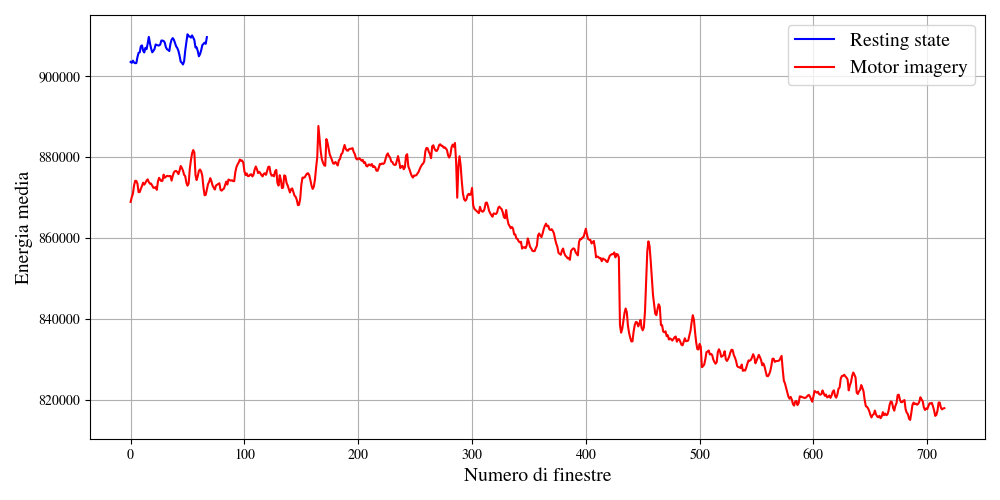
\includegraphics[width=0.8\textwidth]{plot6}
\caption{Confronto tra Resting State e Motor Imagery}
\end{figure}

\end{document}
